In \autoref{sec:pushdown} we showed how to get a pushdown abstraction by separating continuations from the heap that stores values.
%
This separation breaks down when continuations themselves become values via first-class control operators.
%
The glaring issue is that continuations become ``storeable'' and relevant to the execution of functions.
%
But, it was precisely the \emph{irrelevance} that allowed the separation of $\mstore$ and $\mktab$.
%
Specifically, the store components of continuations become elements of the store's codomain --- a recursion that can lead to an unbounded state space and therefore a non-terminating analysis.
%
We apply the AAM methodology to cut out the recursion; whenever a continuation is captured to go into the store, we allocate an address to approximate the store component of the continuation.
%%

%%
We introduce a new environment, $\mmktab$, that maps these addresses to the stores they represent.
%
The stores that contain addresses in $\mmktab$ are then \emph{open}, and must be paired with $\mmktab$ to be \emph{closed}.
%
This poses the same problem as before with contexts in storeable continuations.
%
Therefore, we give up some precision to regain termination by \emph{flattening} these environments when we capture continuations.
%
Fresh allocation still maintains the concrete semantics, but we necessarily lose some ability to distinguish contexts in the abstract.
%%

\subsection{Case study of first-class control: shift and reset}
%%
We choose to study {\tt shift} and {\tt reset}~\citep{ianjohnson:danvy:filinski:delim:1990} because delimited continuations have proven useful for implementing web servers~\citep{dvanhorn:Queinnec2004Continuations,jay-communication}, providing processes isolation in operating systems~\citep{dvanhorn:Kiselyov2007Delimited}, representing computational effects~\citep{dvanhorn:Filinski1994Representing}, modularly implementing error-correcting parsers~\citep{dvanhorn:Shivers2011Modular}, and finally undelimited continuations are \emph{pass\'e} for good reason~\citep{ianjohnson:kiselyov:against-callcc}.
%
Even with all their uses, however, their semantics can yield control-flow possibilities that surprise their users.
%
A \emph{precise} static analysis that illuminates their behavior is then a valuable tool.
%

Our concrete test subject is the abstract machine for shift and reset adapted from \citet{ianjohnson:Biernacki2006274} in the ``{\bf ev}al, {\bf co}ntinue'' style in \autoref{fig:shift-reset}.
%
The figure elides the rules for standard function calls.
%
The new additions to the state space are a new kind of value, $\vcomp{\mkont}$, and a \emph{meta-continuation}, $\mmkont \in \MKont = \Kont^*$ for separating continuations by their different prompts.
%
Composable continuations are indistinguishable from functions, so even though the meta-continuation is concretely a list of continuations, its conses are notated as function composition: $\mkapp{\mkont}{\mmkont}$.

\begin{figure}
  \centering
  $\mstate \stepto_\SR \mstate'$ \\
  \begin{tabular}{r|l}%{r|ll}
    \hline
% Reset
    $\ev{\sreset{\mexpr}, \menv, \mstore,\mkont, \mmkont}$
    &
    $\ev{\mexpr, \menv, \mstore,\epsilon, \mkapp{\mkont}{\mmkont}}$
%    & \textsc{[push prompt]}
    \\
% Pop prompt
    $\co{\epsilon, \mkapp{\mkont}{\mmkont}, \mval,\mstore}$
    &
    $\co{\mkont, \mmkont, \mval,\mstore}$
%    & \textsc{[pop prompt]}
    \\
% Shift
    $\ev{\sshift{\mvar}{\mexpr}, \menv, \mstore,\mkont, \mmkont}$
    &
    $\ev{\mexpr, \extm{\menv}{\mvar}{\maddr},\mstore',\epsilon,\mmkont}$
    \\
    where & $\mstore' = \joinm{\mstore}{\maddr}{\vcomp{\mkont}}$
%    & \textsc{[capture continuation]}
    \\
% continuation call
    $\co{\kcons{\appr{\vcomp{\mkont'}}}{\mkont}, \mmkont, \mval,\mstore}$
    &
    $\co{\mkont', \mkapp{\mkont}{\mmkont}, \mval,\mstore}$
%    & \textsc{[compose continuation]}
    \\
    \text{standard rules} \\
    $\ev{\svar\mvar, \menv, \mstore, \mkont,\mmkont}$
    &
    $\co{\mkont,\mmkont,\mval, \mstore}$ if $\mval \in \mstore(\menv(\mvar))$
    \\
% Application
    $\ev{\sapp{\mexpri0}{\mexpri1},\menv,\mstore,\mkont,\mmkont}$
    &
    $\ev{\mexpri0,\menv,\mstore,\kcons{\appl{\mexpri1,\menv}}{\mkont},\mmkont}$
    \\
% Arg eval
    $\co{\kcons{\appl{\mexpr,\menv}}{\mkont},\mmkont,\mval,\mstore}$
    &
    $\ev{\mexpr,\menv,\mstore,\kcons{\appr{\mval}}{\mkont},\mmkont}$
    \\
% Function call
    $\co{\kcons{\appr{\slam{\mvar}{\mexpr},\menv}}{\mkont},\mmkont,\mval,\mstore}$
    &
    $\ev{\mexpr,\menv',\mstore',\mkont,\mmkont}$ \\
    where & $\menv' = \extm{\menv}{\mvar}{\maddr}$ \\
          & $\mstore' = \joinm{\mstore}{\maddr}{\mval}$
  \end{tabular}  
  \caption{Machine semantics for shift/reset}
  \label{fig:shift-reset}
\end{figure}
%%

\subsection{Reformulated with continuation stores}
%
The machine in \autoref{fig:shift-reset} is transformed now to have three new tables: one for continuations ($\mktab_{\makont}$), one as discussed in the section beginning to close stored continuations ($\mmktab$), and one for meta-continuations ($\mktab_{\mamkont}$).
%
The first is like previous sections, albeit continuations may now have the approximate form that is storeable.
%
The meta-continuation table is more like previous sections because meta-contexts are not storeable.
%
Meta-continuations do not have simple syntactic strategies for bounding their size, so we choose to bound them to size 0.
%
They could be paired with lists of $\sa{Kont}$ bounded at an arbitrary $n \in \nat$, but we simplify for presentation.

Contexts for continuations are still at function application, but now contain $\mmktab$.
%
Contexts for meta-continuations are in two places: manual prompt introduction via {\tt reset}, or via continuation invocation.
%
At continuation capture time, continuation contexts are approximated to remove $\mastore$ and $\mmktab$ components.
%
The different context spaces are thus:
\begin{align*}
  \msctx \in \ExactContext &::= \tpl{\mexpr,\menv,\mastore,\mmktab} \\
  \mactx \in \sa{Context} &::= \tpl{\mexpr,\menv,\maddr} \\
  \mctx \in \Context &::= \mactx \alt \msctx \\
  \mmctx \in \MContext &::= \tpl{\mexpr,\menv,\mastore,\mmktab}
                       \alt \tpl{\mvkont, \maval, \mastore, \mmktab} \\
\end{align*}
%

Revisiting the graphical intuitions of the state space, we have now $\mvkont$ in states' stores, which represent an \emph{overapproximation} of a set of continuations.
%
We augment the illustration from \autoref{fig:pushdown-vis} in \autoref{fig:shiftreset-vis} to include the new $\MKStore$ and the overapproximating behavior of $\mvkont$.
%
The informal notation $\mstore \leadsto \mvkont$ suggests that the state's store \emph{contains}, or \emph{refers to} some $\mvkont$.

\begin{figure}
  \centering
  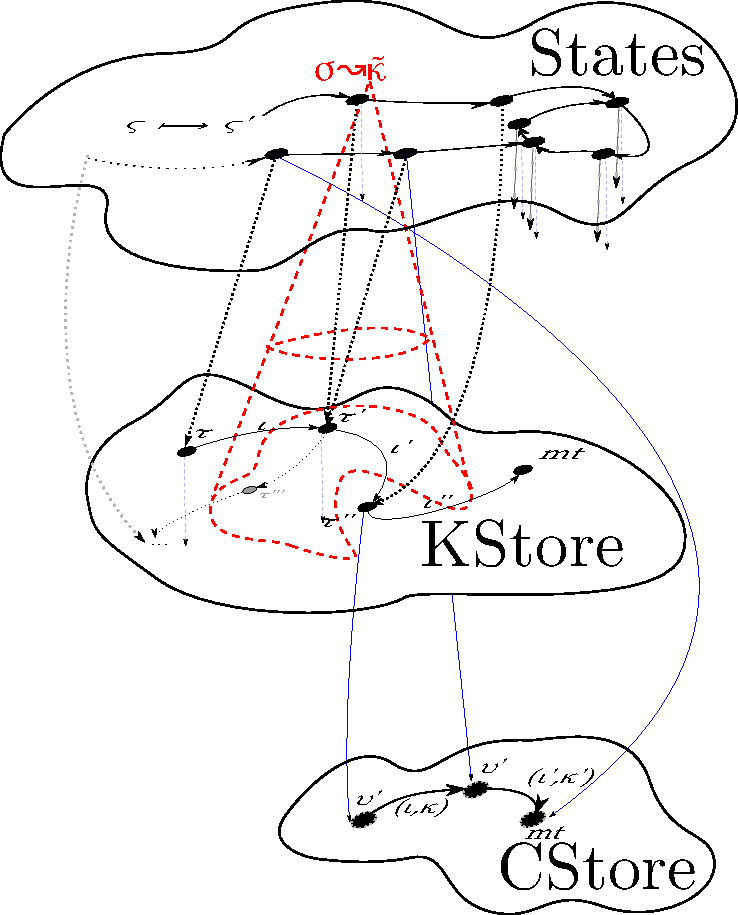
\includegraphics[scale=0.6]{xigraph-approx}
  \caption{Graphical visualization of states, $\mktab_{\makont}$ and $\mktab_{\mamkont}$.}
  \label{fig:shiftreset-vis}
\end{figure}

\begin{figure}
  \centering
  \begin{tabular}{rlrl}
    $\mastate \in \sa{SR}$ &\multicolumn{3}{l}{\hspace{-3mm}$::= \ev{\mexpr,\menv,\mastore,\mmktab,\makont,\mamkont} \alt \co{\makont,\mamkont,\maval,\mastore,\mmktab}$} \\
    $\State$ & \multicolumn{3}{l}{\hspace{-3mm}$::= \mastate,\mktab_{\makont},\mktab_{\mamkont}$} \\
    $\mmktab \in \MKTab$ &\multicolumn{3}{l}{\hspace{-3mm}$= \Addr \finto \wp(\Store)$} \\
    $\mktab_{\makont} \in \KStore$ &\multicolumn{3}{l}{\hspace{-3mm}$= \ExactContext \finto \wp(\sa{Kont})$} \\
    $\mktab_{\mamkont} \in \MKStore$ &\multicolumn{3}{l}{\hspace{-3mm}$= \MContext \finto \wp(\sa{Kont} \times \sa{MKont})$} \\
    $\makont \in \sa{Kont}$ &\hspace{-3mm}$::= \epsilon \alt \kcons{\mkframe}{\mctx} \alt \mctx$ & $\mvkont \in \VKont$ &\hspace{-3mm}$::= \epsilon \alt \mactx$ \\
    $\mamkont \in \sa{MKont}$ &\hspace{-3mm}$::= \epsilon \alt \mmctx$ & $\maval \in \sa{Value}$ &\hspace{-3mm}$::= \mvkont \alt (\mlam,\menv)$
  \end{tabular}
  \caption{Shift/reset abstract semantic spaces}
  \label{fig:shiftreset-spaces}
\end{figure}
%
The approximation and flattening happens in $\approximate$:
\begin{equation*}
  \approximate : \MKTab \times \Addr \times \SKont \to \MKTab \times \VKont
\end{equation*}
\begin{align*}
  \approximate(\mmktab,\maddr,\epsilon) &= \mmktab,\epsilon \\
  \approximate(\mmktab,\maddr,\kcons{\mkframe}{\mctx}) &= \mmktab',\kcons{\mkframe}{\mactx} \text{ where } (\mmktab',\mactx) = \approximate(\mmktab,\maddr,\mctx) \\
  \approximate(\mmktab,\maddr,\tpl{\mexpr,\menv,\mastore,\mmktab'}) &= \joinm{\mmktab\sqcup\mmktab'}{\maddr}{\mastore},\kcons{\mkframe}{\tpl{\mexpr,\menv,\maddr}} \\
  \approximate(\mmktab,\maddr,\tpl{\mexpr,\menv,\maddralt}) &= \joinm{\mmktab}{\maddr}{\mmktab(\maddralt)},\kcons{\mkframe}{\tpl{\mexpr,\menv,\maddr}}
\end{align*}
The third case is where continuation closures get flattened together.
%
The fourth case is when an already approximate continuation is approximated: the approximation is inherited.
%
Approximating the context and allocating the continuation in the store require two addresses, so we relax the specification of $\alloc$ to allow multiple address allocations in this case.

Each of the four rules of the original shift/reset machine has a corresponding rule that we explain piecemeal.
%
We will use $\kindastepto$ for steps that do not modify the continuation stores for notational brevity.
%
We use the above $\approximate$ function in the rule for continuation capture, as modified here.
%
\begin{equation*}\ev{\sshift{\mvar}{\mexpr},\menv,\mastore,\mmktab,\makont,\mamkont} \kindastepto
  \ev{\mexpr,\menv',\mastore',\mmktab',\epsilon,\mamkont}
\end{equation*}
where
\begin{align*}
  (\maddr,\maddr') &= \alloc(\mastate,\mktab_\makont,\mktab_\mamkont) & \menv' &= \extm{\menv}{\mvar}{\maddr} \\
  (\mmktab',\mvkont) &= \approximate(\mmktab,\maddr',\makont) &
  \mastore' &= \joinm{\mastore}{\maddr}{\mvkont}
\end{align*}

The rule for {\tt reset} stores the continuation and meta-continuation in $\mktab_{\mamkont}$:
\begin{align*}
\ev{\sreset{\mexpr},\menv,\mastore,\mmktab,\makont,\mamkont},\mktab_\makont,\mktab_\mamkont &\stepto
  \ev{\mexpr,\menv,\mastore,\mmktab,\epsilon,\mmctx},\mktab_\makont,\mktab_\mamkont' \\
  \text{where } \mmctx &= \tpl{\mexpr,\menv,\mastore,\mmktab} \\
                \mktab_\mamkont &= \joinm{\mktab_{\mamkont}}{\mmctx}{(\makont,\mamkont)}
\end{align*}

The prompt-popping rule simply dereferences $\mktab_{\mamkont}$:
\begin{align*}
  \co{\epsilon,\mmctx,\maval,\mastore,\mmktab} &\kindastepto \co{\makont,\mamkont,\maval,\mastore,\mmktab} \text{ if } (\makont,\mamkont) \in \mktab_{\mamkont}(\mmctx)
\end{align*}

The continuation installation rule extends $\mktab_{\mamkont}$ at the different context:
\begin{align*}
  \co{\makont,\mamkont,\maval,\mastore,\mmktab},\mktab_\makont,\mktab_\mamkont &\stepto \co{\mvkont,\mmctx,\maval,\mastore,\mmktab},\mktab_\makont,\mktab_\mamkont' \\ 
\text{if } & (\appr{\mvkont},\makont') \in \pop(\mktab_{\makont},\mmktab, \makont) \\
\text{where } \mmctx &= \tpl{\mvkont,\maval,\mastore,\mmktab} \\
              \mktab_\mamkont &= \joinm{\mktab_{\mamkont}}{\mmctx}{(\makont',\mamkont)}
\end{align*}
Again we have a metafunction $\pop$, but this time to interpret approximated continuations:
\begin{align*}
  \pop(\mktab_{\makont}, \mmktab, \makont) &= \popaux(\makont,\emptyset) \\
  \text{where } 
   \popaux(\epsilon, G) &= \emptyset \\
   \popaux(\kcons{\mkframe}{\mctx}, G) &= \set{(\mkframe,\mctx)} \\
   \popaux(\mctx, G) &= \bigcup\limits_{\makont \in G'}(\popaux(\makont, G\cup G')) \\
    \text{where } G' &= \bigcup\limits_{\msctx \in I(\mctx)}{\mktab_{\makont}(\msctx)} \setminus G \\
  I(\msctx) &= \set{\msctx} \\
  I(\tpl{\mexpr,\menv,\maddr}) &=
  \setbuild{\tpl{\mexpr,\menv,\mastore,\mmktab'} \in \dom(\mktab_{\makont})}
           {\mastore \in \mmktab(\maddr),
            \mmktab' \sqsubseteq \mmktab}
\end{align*}
Notice that since we flatten $\mmktab$s together, we need to compare for containment rather than for equality (in $I$).
%
A variant of this semantics with GC is available in the PLT redex models.

\paragraph{Comparison to CPS transform to remove {\tt shift} and {\tt reset}:}{
We lose precision if we use a CPS transform to compile away {\tt shift} and {\tt reset} forms, because variables are treated less precisely than continuations.
%
%In pushdown analysis, we track function return points with entire calling contexts rather than the $k$-CFA way of allocating the continuation in the heap at some lower-precision address, like a variable.
%
%In our summarizing analysis of delimited composable control, we get added precision for {\tt reset}, {\tt shift}, and continuation invocation points.
%
Consider the following program and its CPS transform for comparison:
% \begin{lstlisting}[mathescape]
% (let* ([id ($\lambda$ (x) x)]
%        [f ($\lambda$ (y) (shift k (k (k y))))]
%        [g ($\lambda$ (z) (reset (id (f z))))])
%   (<= (g 0) (g 1)))
% \end{lstlisting}
\begin{small}
\begin{SCodeFlow}\begin{RktBlk}\begin{SingleColumn}\RktPn{(}\RktSym{let*}\mbox{\hphantom{\Scribtexttt{x}}}\RktPn{(}\RktPn{[}\RktSym{id}\mbox{\hphantom{\Scribtexttt{x}}}\RktPn{(}\RktSym{$\lambda$}\mbox{\hphantom{\Scribtexttt{x}}}\RktPn{(}\RktSym{x}\RktPn{)}\mbox{\hphantom{\Scribtexttt{x}}}\RktSym{x}\RktPn{)}\RktPn{]}

\mbox{\hphantom{\Scribtexttt{xxxxxxx}}}\RktPn{[}\RktSym{f}\mbox{\hphantom{\Scribtexttt{x}}}\RktPn{(}\RktSym{$\lambda$}\mbox{\hphantom{\Scribtexttt{x}}}\RktPn{(}\RktSym{y}\RktPn{)}\mbox{\hphantom{\Scribtexttt{x}}}\RktPn{(}\RktSym{shift}\mbox{\hphantom{\Scribtexttt{x}}}\RktSym{k}\mbox{\hphantom{\Scribtexttt{x}}}\RktPn{(}\RktSym{k}\mbox{\hphantom{\Scribtexttt{x}}}\RktPn{(}\RktSym{k}\mbox{\hphantom{\Scribtexttt{x}}}\RktSym{y}\RktPn{)}\RktPn{)}\RktPn{)}\RktPn{)}\RktPn{]}

\mbox{\hphantom{\Scribtexttt{xxxxxxx}}}\RktPn{[}\RktSym{g}\mbox{\hphantom{\Scribtexttt{x}}}\RktPn{(}\RktSym{$\lambda$}\mbox{\hphantom{\Scribtexttt{x}}}\RktPn{(}\RktSym{z}\RktPn{)}\mbox{\hphantom{\Scribtexttt{x}}}\RktPn{(}\RktSym{reset}\mbox{\hphantom{\Scribtexttt{x}}}\RktPn{(}\RktSym{id}\mbox{\hphantom{\Scribtexttt{x}}}\RktPn{(}\RktSym{f}\mbox{\hphantom{\Scribtexttt{x}}}\RktSym{z}\RktPn{)}\RktPn{)}\RktPn{)}\RktPn{)}\RktPn{]}\RktPn{)}

\mbox{\hphantom{\Scribtexttt{xx}}}\RktPn{(}\RktSym{$\le$}\mbox{\hphantom{\Scribtexttt{x}}}\RktPn{(}\RktSym{g}\mbox{\hphantom{\Scribtexttt{x}}}\RktVal{0}\RktPn{)}\mbox{\hphantom{\Scribtexttt{x}}}\RktPn{(}\RktSym{g}\mbox{\hphantom{\Scribtexttt{x}}}\RktVal{1}\RktPn{)}\RktPn{)}\RktPn{)}\end{SingleColumn}\end{RktBlk}\end{SCodeFlow}

% \begin{lstlisting}[mathescape]
% (let* ([id ($\lambda$ (x k) (k x))]
%        [f ($\lambda$ (y j) (j (j y)))]
%        [g ($\lambda$ (z h) (h (f z ($\lambda$ (fv) (id fv ($\lambda$ (i) i))))))])
%   (g 0 ($\lambda$ (g0v) (g 1 ($\lambda$ (g1v) (<= g0v g1v))))))
% \end{lstlisting}
\begin{SCodeFlow}\begin{RktBlk}\begin{SingleColumn}\RktPn{(}\RktSym{let*}\mbox{\hphantom{\Scribtexttt{x}}}\RktPn{(}\RktPn{[}\RktSym{id}\mbox{\hphantom{\Scribtexttt{x}}}\RktPn{(}\RktSym{$\lambda$}\mbox{\hphantom{\Scribtexttt{x}}}\RktPn{(}\RktSym{x}\mbox{\hphantom{\Scribtexttt{x}}}\RktSym{k}\RktPn{)}\mbox{\hphantom{\Scribtexttt{x}}}\RktPn{(}\RktSym{k}\mbox{\hphantom{\Scribtexttt{x}}}\RktSym{x}\RktPn{)}\RktPn{)}\RktPn{]}

\mbox{\hphantom{\Scribtexttt{xxxxxxx}}}\RktPn{[}\RktSym{f}\mbox{\hphantom{\Scribtexttt{x}}}\RktPn{(}\RktSym{$\lambda$}\mbox{\hphantom{\Scribtexttt{x}}}\RktPn{(}\RktSym{y}\mbox{\hphantom{\Scribtexttt{x}}}\RktSym{j}\RktPn{)}\mbox{\hphantom{\Scribtexttt{x}}}\RktPn{(}\RktSym{j}\mbox{\hphantom{\Scribtexttt{x}}}\RktPn{(}\RktSym{j}\mbox{\hphantom{\Scribtexttt{x}}}\RktSym{y}\RktPn{)}\RktPn{)}\RktPn{)}\RktPn{]}

\mbox{\hphantom{\Scribtexttt{xxxxxxx}}}\RktPn{[}\RktSym{g}\mbox{\hphantom{\Scribtexttt{x}}}\RktPn{(}\RktSym{$\lambda$}\mbox{\hphantom{\Scribtexttt{x}}}\RktPn{(}\RktSym{z}\mbox{\hphantom{\Scribtexttt{x}}}\RktSym{h}\RktPn{)}
\\\mbox{\hphantom{\Scribtexttt{xxxxxxxxxxx}}}\RktPn{(}\RktSym{h}\mbox{\hphantom{\Scribtexttt{x}}}\RktPn{(}\RktSym{f}\mbox{\hphantom{\Scribtexttt{x}}}\RktSym{z}\mbox{\hphantom{\Scribtexttt{x}}}\RktPn{(}\RktSym{$\lambda$}\mbox{\hphantom{\Scribtexttt{x}}}\RktPn{(}\RktSym{fv}\RktPn{)}
\\\mbox{\hphantom{\Scribtexttt{xxxxxxxxxxxxxxxxxxxx}}}\RktPn{(}\RktSym{id}\mbox{\hphantom{\Scribtexttt{x}}}\RktSym{fv}\mbox{\hphantom{\Scribtexttt{x}}}\RktPn{(}\RktSym{$\lambda$}\mbox{\hphantom{\Scribtexttt{x}}}\RktPn{(}\RktSym{i}\RktPn{)}\mbox{\hphantom{\Scribtexttt{x}}}\RktSym{i}\RktPn{)}\RktPn{)}\RktPn{)}\RktPn{)}\RktPn{)}\RktPn{)}\RktPn{]}\RktPn{)}

\mbox{\hphantom{\Scribtexttt{xx}}}\RktPn{(}\RktSym{g}\mbox{\hphantom{\Scribtexttt{x}}}\RktVal{0}\mbox{\hphantom{\Scribtexttt{x}}}\RktPn{(}\RktSym{$\lambda$}\mbox{\hphantom{\Scribtexttt{x}}}\RktPn{(}\RktSym{g0v}\RktPn{)}\mbox{\hphantom{\Scribtexttt{x}}}\RktPn{(}\RktSym{g}\mbox{\hphantom{\Scribtexttt{x}}}\RktVal{1}\mbox{\hphantom{\Scribtexttt{x}}}\RktPn{(}\RktSym{$\lambda$}\mbox{\hphantom{\Scribtexttt{x}}}\RktPn{(}\RktSym{g1v}\RktPn{)}\mbox{\hphantom{\Scribtexttt{x}}}\RktPn{(}\RktSym{$\le$}\mbox{\hphantom{\Scribtexttt{x}}}\RktSym{g0v}\mbox{\hphantom{\Scribtexttt{x}}}\RktSym{g1v}\RktPn{)}\RktPn{)}\RktPn{)}\RktPn{)}\RktPn{)}\RktPn{)}\end{SingleColumn}\end{RktBlk}\end{SCodeFlow}
\end{small}
The $\CESKKstart$ machine with a monovariant allocation strategy will predict the CPS'd version returns true or false.
%
In analysis literature, ``monovariant'' means variables get one address, namely themselves.
%
Our specialized analysis for delimited control will predict the non-CPS'd version returns true.}

\iftr{
\subsection{Correctness}
We impose an order on values since stored continuations are more approximate in the analysis than in $\SR$:
\begin{mathpar}
  \inferrule{ }{\mval \sqsubseteq_{\mktab,\mmktab} \mval} \quad
  \inferrule{\mkont \sqsubseteq \unroll{\mktab,\mmktab}{\mvkont}}
            {\vcomp{\mkont} \sqsubseteq_{\mktab,\mmktab} \mvkont} \quad
  \inferrule{\forall \mval\in\mstore(\maddr).
             \exists \maval\in\mastore(\maddr).
             \mval \sqsubseteq_{\mktab,\mmktab} \maval}
            {\mstore \sqsubseteq_{\mktab,\mmktab} \mastore} \\
  \inferrule{\mkont \sqsubseteq \unroll{\mktab_{\makont},\mmktab}{\makont} \\
             \mmkont \sqsubseteq \unrollC{\mktab_{\makont},\mktab_{\mamkont},\mmktab}{\mamkont} \\
             \mstore \sqsubseteq_{\mktab_{\makont},\mmktab} \mastore}
            {\ev{\mexpr,\menv,\mstore,\mkont,\mmkont} \sqsubseteq
             \ev{\mexpr,\menv,\mastore, \mmktab,\makont,\mamkont}, \mktab_{\makont}, \mktab_{\mamkont}} \\
  \inferrule{\mval \sqsubseteq_{\mktab_{\makont},\mmktab} \maval \\
             \mkont \sqsubseteq \unroll{\mktab_{\makont},\mmktab}{\makont} \\
             \mmkont \sqsubseteq \unrollC{\mktab_{\makont},\mktab_{\mamkont},\mmktab}{\mamkont} \\
             \mstore \sqsubseteq_{\mktab_{\makont},\mmktab} \mastore}
            {\co{\mkont,\mmkont,\mval,\mstore} \sqsubseteq
             \co{\makont,\mamkont,\maval,\mastore, \mmktab}, \mktab_{\makont}, \mktab_{\mamkont}}
\end{mathpar}
Unrolling differs from the previous sections because the values in frames can be approximate.
%
Thus, instead of expecting the exact continuation to be in the unrolling, we have a judgment that an unrolling approximates a given continuation in \autoref{fig:cont-order} (note we reuse $I$ from $\popaux$'s definition).

\begin{figure}
  \centering
  \begin{mathpar}
    \inferrule{ }{\appl{\mexpr,\menv} \sqsubseteq_{\mktab,\mmktab}
      \appl{\mexpr,\menv}} \quad \inferrule{\mval
      \sqsubseteq_{\mktab,\mmktab}{\maval}}
    {\appr{\mval} \sqsubseteq_{\mktab,\mmktab} \appr{\maval}} \\
    \inferrule{ }{\epsilon \sqsubseteq
      \unroll{\mktab,\mmktab}{\epsilon}} \quad
    \inferrule{\mkframe \sqsubseteq_{\mktab,\mmktab} \makframe \\
      \mkont \sqsubseteq \unroll{\mktab,\mmktab}{\mctx}}
    {\kcons{\mkframe}{\mkont} \sqsubseteq
      \unroll{\mktab,\mmktab}{\kcons{\makframe}{\mctx}}}
    \\
    \inferrule{\makont \in \mktab(\msctx) \quad
      \mkont \sqsubseteq \unroll{\mktab,\mmktab}{\makont}} {\mkont
      \sqsubseteq \unroll{\mktab,\mmktab}{\msctx}}
    \quad
    \inferrule{\msctx \in I(\mktab,\mmktab,\mactx) \quad
      \mkont \sqsubseteq \unroll{\mktab,\mmktab}{\msctx}} {\mkont
      \sqsubseteq \unroll{\mktab,\mmktab}{\mactx}}
    \\
    \inferrule{ }
              {\epsilon \sqsubseteq \unrollC{\mktab_{\makont},\mktab_{\mamkont},\mmktab}{\epsilon}}
    \\
    \inferrule{(\makont,\mamkont) \in \mktab_{\mamkont}(\mmctx) \\
               \mkont \sqsubseteq \unroll{\mktab_{\makont},\mmktab}{\makont} \\
               \mmkont \sqsubseteq \unrollC{\mktab_{\makont},\mktab_{\mamkont},\mmktab}{\mamkont}}
              {\mkapp{\mkont}{\mmkont} \sqsubseteq \unrollC{\mktab_{\makont},\mktab_{\mamkont},\mmktab}{\mmctx}}
  \end{mathpar}
  
  \caption{Order on (meta-)continuations}
\label{fig:cont-order}
\end{figure}
\begin{theorem}[Soundness]
  If $\somestate \stepto_{\SR} \nextstate$, and $\somestate \sqsubseteq \someotherstate$ then there is $\nextotherstate$ such that $\someotherstate \stepto_{\SRSChKKt} \nextotherstate$ and
$\nextstate \sqsubseteq \nextotherstate$.
\end{theorem}

\paragraph{Freshness implies completeness}
The high level proof idea is that fresh allocation separates evaluation into a sequence of bounded length paths that have the same store, but the store only grows and distinguishes contexts such that each continuation and metacontinuation have a unique unrolling.
%
It is an open question whether the addition of garbage collection preserves completeness.
%
Each context with the same store will have different expressions in them since expressions can only get smaller until a function call, at which point the store grows.
%
This forms an order on contexts: smaller store means smaller context, and same store but smaller expression (indeed a subexpression) means a smaller context.
%
Every entry in each enviroment ($\mastore,\mmktab,\mktab_\makont,\mktab_\mamkont$) will map to a unique element, and the continuation stores will have no circular references (the context in the tail of a continuation is strictly smaller than the context that maps to the continuation).
%
There can only be one context that $I$ maps to for approximate contexts because of the property of stores in contexts.

We distill these intuitions into an invariant about states that we will then use to prove completeness.
%
\begin{mathpar}
  \inferrule{\forall \maddr\in\dom(\mastore).\exists \maval. \mastore(\maddr)=\set{\maval}\wedge\maval\preceq_\mmktab\mktab_\makont \\
    \forall \maddr\in\dom(\mmktab).\exists\mastore'.\mmktab(\maddr) =\set{\mastore'}\wedge\mastore'\in\pi_3(\dom(\mktab_\makont)) \\
    \forall \msctx\in\dom(\mktab_\makont).\exists\makont. \mktab_\makont(\msctx) = \set{\makont}\wedge \makont \sqsubset_\mmktab^{\mktab_\makont} \msctx\\
    \forall \mmctx\in\dom(\mktab_\mamkont).\exists\mamkont.\mktab_\mamkont(\mmctx) = \set{\mamkont}\wedge \mamkont \sqsubset \mmctx \\
}{\inv^*(\mastore, \mmktab, \mktab_{\makont}, \mktab_{\mamkont})}
 \\
\inferrule{\inv^*(\mastore,\mmktab,\mktab_\makont,\mktab_\mamkont) \\
           \tpl{\mexpr,\menv,\mastore,\mmktab} \sqsubset \dom(\mktab_\makont) \cup \dom(\mktab_\mamkont) \\
           (\exists \tpl{\mexpr_c,\menv,\mastore,\mmktab} \in \dom(\mktab_\makont)) \implies \mexpr \in \mathit{subexpressions}(\mexpr_c) \\
           \makont \preceq_\mmktab \mktab_\makont \\
           \mamkont \preceq \mktab_\mamkont}
          {\inv_\fresh(\ev{\mexpr,\menv,\mastore,\mmktab,\makont,\mamkont},\mktab_\makont,\mktab_\mamkont)} \\
\inferrule{\inv^*(\mastore,\mmktab,\mktab_\makont,\mktab_\mamkont) \\
           \maval \preceq_\mmktab \mktab_\makont \\
           \makont \preceq_\mmktab \mktab_\makont \\
           \mamkont \preceq \mktab_\mamkont}
          {\inv_\fresh(\co{\makont,\mamkont,\maval,\mastore,\mmktab},\mktab_\makont,\mktab_\mamkont)}
\end{mathpar}
Where the order $\preceq$ states that any contexts in the (meta-)continuation are mapped in the given table.
\begin{mathpar}
  \inferrule{ }{(\mlam,\menv) \preceq_\mmktab \mktab_\makont} \quad
  \inferrule{ }{\epsilon \preceq_\mmktab \mktab_\makont} \quad
  \inferrule{ }{\epsilon \preceq \mktab_\mamkont} \quad
  \inferrule{\msctx \in \dom(\mktab_\makont)}{\msctx\preceq_\mmktab \mktab_\makont} \quad
  \inferrule{\mmctx \in \dom(\mktab_\mamkont)}{\mmctx \preceq \mktab_\mamkont}\\
  \inferrule{\exists\mastore.\mmktab(\maddr)=\set{\mastore} \\
             \exists!\mmktab'.\tpl{\mexpr,\menv,\mastore,\mmktab'} \in\dom(\mktab_\makont)\wedge\mmktab' \sqsubseteq \mmktab
           }
            {\tpl{\mexpr,\menv,\maddr} \preceq_\mmktab \mktab_\makont}
\end{mathpar}
And the order $\sqsubset$ states that the contexts in the (meta-)continuation are strictly smaller than the given context.
\begin{mathpar}
  \inferrule{ }{\epsilon \sqsubset_\mmktab^{\mktab_{\makont}}} \quad \inferrule{ }{\epsilon \sqsubset \mmctx} \quad \inferrule{\mctx \sqsubset_\mmktab^{\mktab_\makont} \msctx}{\kcons{\mkframe}{\mctx} \sqsubset_\mmktab^{\mktab_\makont} \msctx} \\
  \inferrule{\mexpr' \in \mathit{subexpressions}(\mexpr)}{\tpl{\mexpr',\menv,\mastore,\mmktab} \sqsubset_\mmktab^{\mktab_\makont} \tpl{\mexpr,\menv,\mastore,\mmktab}} \quad
  \inferrule{\mexpr' \in \mathit{subexpressions}(\mexpr)}{\tpl{\mexpr',\menv,\mastore,\mmktab} \sqsubset \tpl{\mexpr,\menv,\mastore,\mmktab}} \\
  \inferrule{\dom(\mastore) \sqsubset \dom(\mastore')}{\tpl{\_,\_,\mastore,\_} \sqsubset_\mmktab^{\mktab_\makont} \tpl{\_,\_,\mastore',\_}} \quad
  \inferrule{\dom(\mastore) \sqsubset \dom(\mastore')}{\tpl{\_,\_,\mastore,\_} \sqsubset \tpl{\_,\_,\mastore',\_}} \\
  \inferrule{\forall \msctx' \in I(\mktab_\makont,\mmktab,\mactx) \\ \msctx' \sqsubset_\mmktab^{\mktab_\mkont} \msctx}{\mactx \sqsubset_\mmktab^{\mktab_\makont} \msctx}
\end{mathpar}

\begin{lemma}[Freshness invariant]
  If $\alloc$ produces fresh addresses, $\inv_{\fresh}(\mastate,\mktab_\makont,\mktab_\mamkont)$ and
$\mastate,\mktab_{\makont},\mktab_{\mamkont} \stepto
\mastate',\mktab'_{\makont},\mktab'_{\mamkont}$ then
$\inv_{\fresh}(\mastate',\mktab'_{\makont},\mktab'_{\mamkont})$.
\end{lemma}
\begin{proof}
  By case analysis on the step.
\end{proof}
\begin{theorem}[Complete for fresh allocation]
  If $\alloc$ produces fresh addresses then the resulting semantics is complete with respect to states satisfying the invariant.
\end{theorem}
\begin{proof}[Proof sketch]
  By case analysis and use of the invariant to exploit the fact the unrollings are unique and the singleton codomains pigeon-hole the possible steps to only concrete ones.
\end{proof}
}
%  LocalWords:  pushdown storeable codomain AAM ianjohnson Kiselyov
%  LocalWords:  modularly parsers undelimited Biernacki ev al ntinue
%  LocalWords:  Composable dereferences metafunction timestamped
%  LocalWords:  timestamp codomains
